% 9 variables in here:
% h_1 = 1000.0, h_2 = 1002.0, h_3 = 997.0, ux_1 = 0.0, ux_2 = 0.0, ux_3 = 0.0, uy_1 = 0.0, uy_2 = 0.0, uy_3 = 0.0
\begin{figure}[h!]
\centering
  \subfloat[Height values $h_2 = 12$ and $h_3=7$, all momentums are 0. The variable $h_1$ ranges from 8 to 12.] {
    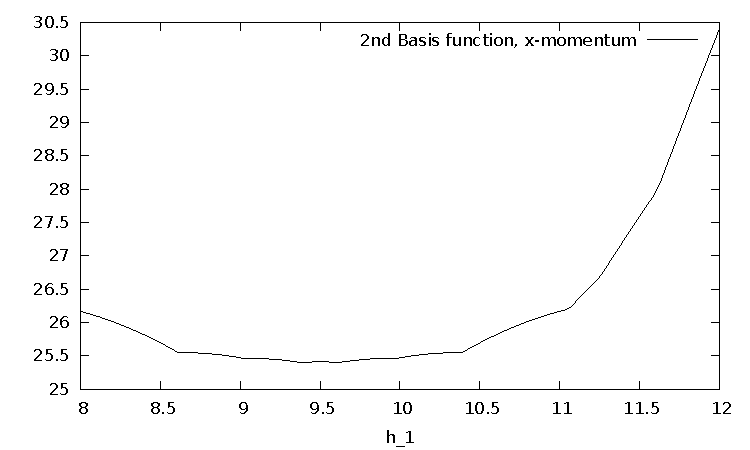
\includegraphics[scale=\zoomfactor]{{{magnitude_10_nonstd/y_12.0_7.0_0.0_0.0_0.0_0.0_0.0_0.0f02}}}
  }
  \subfloat[Height values $h_2 = 1002$ and $h_3=997$, all momentums are 0. The variable $h_1$ ranges from 8 to 12.] {
    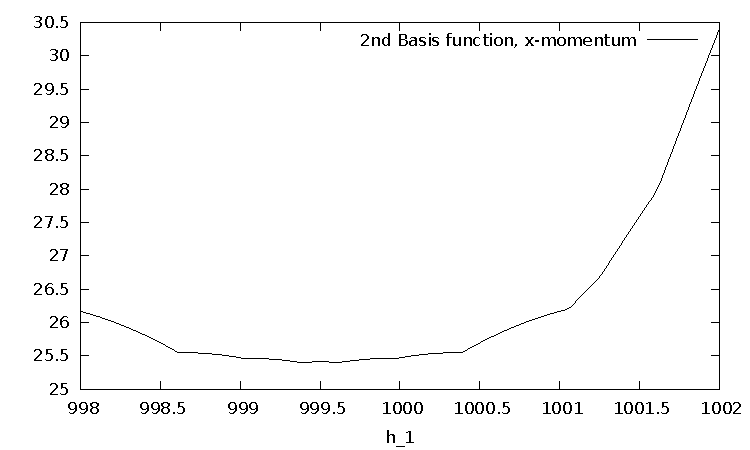
\includegraphics[scale=\zoomfactor]{{{magnitude_1000_nonstd/y_1002.0_997.0_0.0_0.0_0.0_0.0_0.0_0.0f02}}}
  }
\caption{Comparison of different orders of magnitudes for differing height values.}
\label{fig:magnitude_comparison_differing_heights}
\end{figure}

%%% Local Variables:
%%% TeX-master: "../results.tex"
%%% End:
